\documentclass[a4paper, 9pt, twocolumn]{extarticle}
\usepackage{amsmath,graphicx,amssymb,cite}
\usepackage[utf8]{inputenc}
\usepackage[english]{babel}

\usepackage{url}
\usepackage{hyperref}


\addtolength{\textwidth}{2.1cm}
\addtolength{\topmargin}{-2.4cm}
\addtolength{\oddsidemargin}{-1.1 cm}
\addtolength{\textheight}{4.5cm}
\setlength{\columnsep}{0.7cm}

% User defined macros
\def\x{{\mathbf x}}
\def\L{{\cal L}}
\def\SM{{\mathcal S}}
\def\SMO{{\mathcal S^{\mathrm{chroma}}}}
\def\SMS{{\mathcal S^{\mathrm{enh}}}}
\def\SMP{{\mathcal S^{\mathrm{path}}}}
\def\SMPI{{\mathcal S^{\mathrm{struct}}}}
%\def\SMPC{{\mathcal S^{\mathrm{pc}}}}
\def\SMPC{{\mathcal S^{\mathrm{pb}}}}

\pagestyle{empty}

\begin{document}

\date{\normalsize 12.01.2025}

\title{\vspace{-8mm}\textbf{\Large
Chord Recognition\footnote{This is the summary for the reading assignment,
which is part of the exercise of the lecture \emph{Music Processing Analysis}, Winter Term 2023/24,
Friedrich-Alexander Universit\"at Erlangen-N\"urnberg.
Instructor: Prof.\ Dr.\ Meinard M\"uller,
Tutor: Simon Schw\"ar.
}}}

% Hier die Namen und Daten der beteiligten Autoren eintragen
\author{
{
\begin{minipage}{\textwidth}
\center
Quang Hoang Nguyen Vo \\
\small
Friedrich-Alexander University\"at Erlangen-N\"urnberg
\protect\\{} %
\url{quang.nguyen.vo@FAU.de}
\end{minipage}
}
}

\maketitle
\thispagestyle{empty}

%%%%%%%%%%%%%%%%%%%%%%%%%%%%%%%%%%%%%%%%%%%%%%%%%%%%%%%%%%%%%%%%%%%%%%%%%%%%%%
\section{Introduction}
\label{section:introduction}
%%%%%%%%%%%%%%%%%%%%%%%%%%%%%%%%%%%%%%%%%%%%%%%%%%%%%%%%%%%%%%%%%%%%%%%%%%%%%%

In music, harmony is the backbone of a piece. It is the concept of combining different sound together in order to create a cohesive sound to the listener.
The most fundamental building block of harmony, at least in Western music, is the chord. A chord is a set of notes played simultaneously, usually consisting of three or more notes. The most basic type of chord is the triad, which consists of three notes played together.

Harmony analysis can be as well regarded as the study of the relationship and progression of chords in a piece of music. It is a crucial part of music theory and is essential for understanding the structure of a piece of music. In this summary, we will discuss the basic theory of harmony, as well as two methods for automatic chord recognition: template-based chord recognition in section \ref{section:template_recognition} and HMM-based chord recognition in section\ref{section:HMM_recognition}.


%%%%%%%%%%%%%%%%%%%%%%%%%%%%%%%%%%%%%%%%%%%%%%%%%%%%%%%%%%%%%%%%%%%%%%%%%%%%%%
\section{Basic Theory of Harmony}
\label{section:theory}
%%%%%%%%%%%%%%%%%%%%%%%%%%%%%%%%%%%%%%%%%%%%%%%%%%%%%%%%%%%%%%%%%%%%%%%%%%%%%%
%%%%%%%%%%%%%%%%%%%%%%%%%%%%%%%%%
\subsection{Intervals}
\label{subsection:intervals}
%%%%%%%%%%%%%%%%%%%%%%%%%%%%%%%%%
In music theory, an interval is the difference in frequency between two pitches or notes. One of the most basic intervals is the octave, which is the interval between two pitches where one pitch has twice or half the frequency of the other.
With this basic interval, we can build other intervals by taking frequency, geometric or note relations into account.
For Western music, which uses twelve-tone equal temperament, there are twelve basic intervals, which are the semitones. Semitones is defined as the interval between two adjacent notes on the chromatic scale. The chromatic scale is a scale that consists of twelve notes, each a semitone apart from the next. \emph{Figure~\ref{figure:intervals}} illustrates the name of the intervals.

%%%%%%%%%%%%%%%%%%%%%%%%%%%%%%%%%
\subsection{Triads}
\label{subsection:triads}
%%%%%%%%%%%%%%%%%%%%%%%%%%%%%%%%%
In Western music, the most basic type of chord is the triad, which consists of three notes played together.
The first note is called the root note, which gives the chord its name. The second and third note are called the third and the fifth, respectively. Since there are minor thirds, major thirds and augmented fifths, we can distinguish 4 types of different triads: major, minor, diminished and augmented.
The major triads, consisting of a root note a major third and a perfect fifth, are often associated with a happy or bright sound. The minor triads, on the other hand, swap a major third for a minor third. They are often associated with a sad or melancholic sound. \emph{Figure~\ref{figure:triads}} illustrates the major and minor triads. Asides from the major and minor triads, there are also other types of triads, such as the diminished triad and the augmented triad.
Diminished triad consists of a root note, a minor third, and a diminished fifth; meanwhile the augmented chord have a root note, a major third, and an augmented fifth. Both of these triads have a more dissonant sound compared to the major and minor triads, and are often used to create tension in music.

%%%%%%%%%%%%%%%%%%%%%%%%%%%%%%%%%
\subsection{Major and Minor Chords}
\label{subsection:major_minor}
%%%%%%%%%%%%%%%%%%%%%%%%%%%%%%%%%
With 12 notes on chromatic scale, we can build 24 major and minor chords with 12 for each type. \emph{Figure~\ref{figure:chords}} illustrates the 24 major and minor chords. A chord takes the name of its root note. So a root note of A will have a chord \textbf{A}. The major chord is denoted by the chord name, while the minor chord is denoted by the chord name followed by a lowercase \textbf{m}. For example, the major chord with the root note of A is denoted as \textbf{A}, while the minor chord with the root note of A is denoted as \textbf{Am}.
There are several various way to realising a chord, such as root position, first inversion and second inversion. The root position is when the root note is the lowest note in the chord. The first inversion is when the third note is the lowest note in the chord. The second inversion is when the fifth note is the lowest note in the chord. Besides those exists the broken chord or arpeggio, which is when the notes of the chord are played one after the other instead of simultaneously. 




%%%%%%%%%%%%%%%%%%%%%%%%%%%%%%%%%%%%%%%%%%%%%%%%%%%%%%%%%%%%%%%%%%%%%%%%%%%%%%
\section{Template-based Chord Recognition}
\label{section:template_recognition}
%%%%%%%%%%%%%%%%%%%%%%%%%%%%%%%%%%%%%%%%%%%%%%%%%%%%%%%%%%%%%%%%%%%%%%%%%%%%%%
One of the straighforward method for chord recognition is using pattern matching. Given the chroma sequence $X = (x_1, x_2, \ldots, x_N)$, and a set $\Lambda$ of possible chord labels, the task is to assign each chroma vector $x_n \in \mathbb{R}^{12}$ to a chord label $\lambda in \Lambda$.

There are without a doubt several limitations when performing  One of them are due to ambiguity in the chords, acoustic noise or the difference in tunning.


%%%%%%%%%%%%%%%%%%%%%%%%%%%%%%%%%%%%%%%%%%%%%%%%%%%%%%%%%%%%%%%%%%%%%%%%%%%%%%
\section{HMM-Based Chord Recognition}
\label{section:HMM_recognition}
%%%%%%%%%%%%%%%%%%%%%%%%%%%%%%%%%%%%%%%%%%%%%%%%%%%%%%%%%%%%%%%%%%%%%%%%%%%%%%
Chord progression in music are not arbitary, but rather follow a certain rules. Therefore, one may find that the chord that is being played at a given time is dependent on the chord that was played before. This dependency can be modelled using Hidden Markov Models (HMMs).
%%%%%%%%%%%%%%%%%%%%%%%%%%%%%%%%%
\subsection{Markov Chains and Transition Probabilities}
\label{subsection:Markov_chain}
%%%%%%%%%%%%%%%%%%%%%%%%%%%%%%%%%
In order to generalise the task, given a set of states of size $l \in N$

\begin{equation}
    \mathcal{A} := \{\alpha_1, \alpha_2, \ldots, \alpha_l\},
\end{equation}

consisting of distinct elements $\alpha_i$ for $i \in [1:l]$, also known as \textbf{states}.
A chord progression can be modelled as a system that can be described at any time instances $n \in N$ by a state $S_n \in \mathcal{A}$.
For simplicity, assumption is made that the system is memoryless, meaning that the state at time $n$ is only dependent on the state at time $n-1$, this property is expressed as a conditional probability

\begin{equation}
    P(S_n | S_{n-1}, S_{n-2}, \ldots, S_1) = P(S_n | S_{n-1}).
\end{equation}

Other assumptions includes the system is stationary, so the system is invariant under time shifts. Hence the state transition probability $a_{ij}$ is independent of time $n$ and only depends on the states $S_i$ and $S_j$. 
\begin{equation}
    a_{ij} := P(S_n | S_{n-1}) = P(S_2 | S_1).
\end{equation}
Needless to say these coefficients follow standard probability constraint
\begin{equation}
    \sum_{j=1}^{l} a_{ij} = 1.
\end{equation}

A system that satisfies these properties are called a Markov chain. \emph{Figure~\ref{figure:markov_chain}} illustrates a chord progression Markov chain with 3 states.


%%%%%%%%%%%%%%%%%%%%%%%%%%%%%%%%%
\subsection{Hidden Markov Models}
\label{subsection:HMM}
%%%%%%%%%%%%%%%%%%%%%%%%%%%%%%%%%
Based on Markov chain, we extend the concept to Hidden Markov Models (HMMs). Unlike Markov chain, the state sequence is no longer directly observable, hence the name "hidden". Instead, each state can emit entities that are visible to the outside world. As an analogue, we can see the hidden states are the unidentified chord, while the observations are the chroma features of the audio at a given time.

Formally, an HMM is defined by
a sequence of hidden states $\mathcal{A} = \{\alpha_1, \alpha_2, \ldots, \alpha_l\}$, a probability matrix $A = [a_{ij\in [1:l]}]$ of state transition probabilities and vector $C = (c_1, c_2, \ldots, c_l)$ of initial state probabilities.
In case of \textbf{discrete HMM}, the emission space is assumed to be a finite set
\begin{equation}
    \mathcal{B} = \{\beta_1, \beta_2, \ldots, \beta_K\},
\end{equation}
of size $K \in N$. The emission probability matrix $B = [b_{jk}]$ is defined as the probability of emitting observation $\beta_k$ in state $\alpha_j$, it also satisfies the probability constraint like the transition matrix.
In general, a (discrete) HMM is defined by the tuple
\begin{equation}
    \Theta = (\mathcal{A}, A, C, \mathcal{B}, B).
\end{equation}

%%%%%%%%%%%%%%%%%%%%%%%%%%%%%%%%%
\subsection{Uncovering}
\label{subsection:implementation}
%%%%%%%%%%%%%%%%%%%%%%%%%%%%%%%%%
The task of chord recognition can be seen as an \textbf{uncovering problem}.
Given an input sequence of observation $O = (o_1, o_2, \ldots, o_M)$ and a HMM $\Theta$, the goal is to find the most likely sequence of hidden states $S = (s_1, s_2, \ldots, s_M)$ that generated the observation sequence.

One solution for such problem is a brute force way, where one compute the probability of all possible sequences of hidden states and select the sequence with the highest probability. However, this is computationally infeasible, as its comlexity is exponential in the number of hidden states.

Instead, we can use the Viterbi algorithm to find the most likely sequence of hidden states given the observed states. Viterbi algorithm is a dynamic programming algorithm that computes the most likely sequence of hidden states in a HMM. 
The idea is to compute the optimal path to each state at each time step, then use this information to compute the optimal path to the next state.
\begin{equation}
    \delta(i, n) := \max_{(s_1, \ldots ,s_{n})} P[O(1:n), (s_1, s_2, \ldots, s_{n-1}, s_n = \alpha_i)| \Theta].
\end{equation}
$\delta(i,n)$ is highest probability along a single state sequnece $(s_1, \ldots, s_n)$ that ends in state $\alpha_i$ and generates the observation sequence $O(1:n)$. Then the solution is the state sequence or path that yields the maximum value of $\delta(i,n)$. The matrix $\delta$ can be computed recursively as follows
\begin{equation}
    \delta(i, n) = \max_{j \in [1:l]} (\delta(j, n-1) a_{ji} )b_{ik_n}.
\end{equation}
After finding the state sequence, we need to perform \textbf{backtracking} to find the most likely sequence of hidden states. Let $S^*$ be the optimal state sequence, then  the last element $\alpha_{iN}$ is determined by 
\begin{equation}
    i_N = \arg \max_{j \in [1:l]} \delta(j, N).
\end{equation}

% %%%%%%%%%%%%%%%%%%%%%%%%%%%%%%%%%%%%%%%%%%%%%%%%%%%%%%%%%%%%%%%%%%%%%%%%%%%%%%
% \section{Conclusion}
% \label{section:conclusion}
% %%%%%%%%%%%%%%%%%%%%%%%%%%%%%%%%%%%%%%%%%%%%%%%%%%%%%%%%%%%%%%%%%%%%%%%%%%%%%%

%%%%%%%%%%%%%%%%%%%%%%%%%%%%%%%%%%%%%%%%%%%%%%%%%%%%%%%%%%%%%%%%%%%%%%%%%%%%%%
% Here you find some additional LaTex code fragments for including figures and
% references which you may find helpful.
%%%%%%%%%%%%%%%%%%%%%%%%%%%%%%%%%%%%%%%%%%%%%%%%%%%%%%%%%%%%%%%%%%%%%%%%%%%%%%

Example for a citation:~\cite{Mueller21_FMP_SPRINGER}.

Example for figure: Figure~\ref{figure:example}.

\newpage

%%%%%%%%%%%%%%%%%%%%%%%%%%%%%%%%%%%%%%%%%%%%%%%%%%%%%%%%%%%%%%%%%%%%%%%%%%%%%%
\section{Feedback}
\label{section:feedback}
%%%%%%%%%%%%%%%%%%%%%%%%%%%%%%%%%%%%%%%%%%%%%%%%%%%%%%%%%%%%%%%%%%%%%%%%%%%%%%


%-----------------------
\begin{figure}[t]
    \centering
    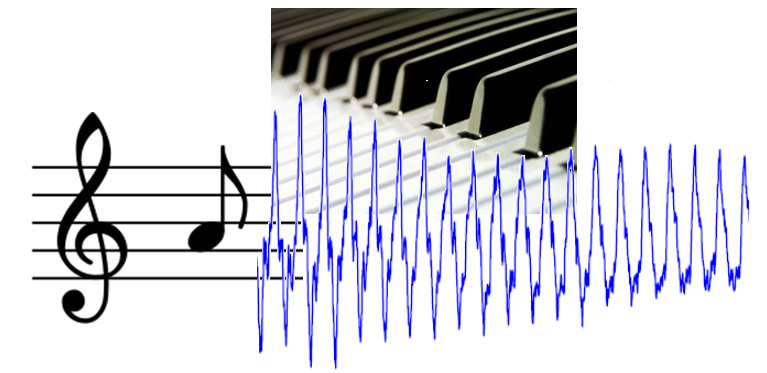
\includegraphics[width=5cm]{figure_example.png}
    \caption{Example for a figure.}
    \label{figure:example}
\end{figure}
%-----------------------


% Feedback may also be given in form of bullet points
% \begin{itemize}
%     \item This was good....
%     \item I did not like...
% \end{itemize}



%%%%%%%%%%%%%%%%%%%%%%%%%%%%%%%%%%%%%%%%%%%%%%%%%%%%%%%%%%%%%%%%%%%%%%%%%%%%%%%%%%%%%%%%%%%%%%%%%%
\bibliographystyle{abbrv}
\small
\bibliography{references}
%%%%%%%%%%%%%%%%%%%%%%%%%%%%%%%%%%%%%%%%%%%%%%%%%%%%%%%%%%%%%%%%%%%%%%%%%%%%%%%%%%%%%%%%%%%%%%%%%%



\end{document}
